\section{Returning results to the client}
\label{sec:visitor}

As mentioned in \cref{sec:overview} every command implementing the
``IReplCommand'' interface should return an instance of a class implementing an
``IResult'', after which it is up to the implementing client to determine how
to display the result. Since commands can fail or result in an exception (see
\cref{sec:function-comp}) it is not always clear what kind of ``IResult'' the
command will return.

To illustrate this it is certainly possible that a user tries to evaluate an
input that passes the parsing step but fails with an exception at the analyze
step (\cref{fig:unit-flow}).  The expected result is an ``EvaluateResult'', but
we can not create the corresponding wrapped ``AnalyzeUnit'' since only an
exception was thrown.

To solve this problem the visitor pattern has been adopted. As can be seen in
\cref{fig:uml-visitor} every ``IResult'' can be ``visited'' by classes
implementing the ``IResultVisitor'' interface. Any class implementing the
``IResultVisitor'' can then decide per result type how to display the returned
information. Since all commands can always return a result with the original
exception or failed ``ISpoofaxResult'', the client is always provided with
error messages as well as the results of earlier processing steps.

\begin{figure}[h]
  \centering
  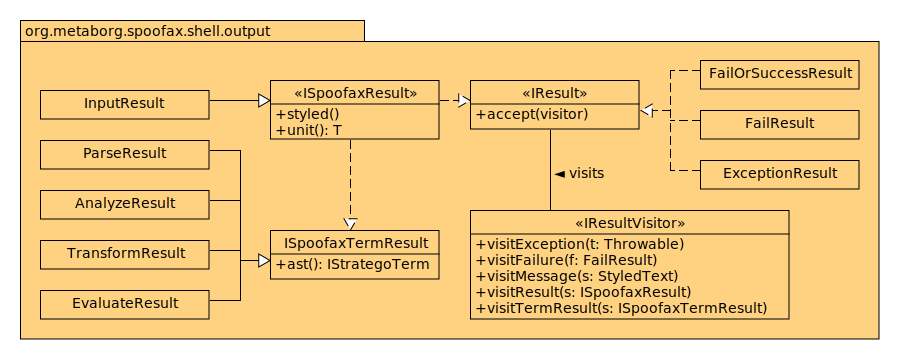
\includegraphics[width=0.8\textwidth]{uml-visitor}
  \caption{UML of the various concrete results and of the result visitor.}
  \label{fig:uml-visitor}
\end{figure}

The client then has the responsibility to decide how to present the returned
data to the user, resulting in a lot of flexibility with regards to displaying.
For a text based console REPL this flexibility is not always necessary, but it
can be used to easily highlight errors or print stack traces. When integrating
the REPL inside Eclipse's GUI toolkit this flexibility was however very useful.
